\section{Stokes equations}
The Stokes equation or, more generally, the Navier-Stokes equation describes a fluid flow. The required functions in the equation are the vector field of fluid velocities and the scalar pressure field. The difficulty in solving this problem lies in the fact that the equations themselves are non-linear, which immediately indicates the use of iterative methods for solving the resulting system of algebraic equations. More than that, the solution of such equations reduces to finding the Jacobi matrix, or even the Hessian matrix. These matrices are relatively easy to find and work with, in the case where the number of equations and variables is small, but in practice using non-trivial methods of constructing a discrete space leads to hundreds of thousands of variables. Another point complicating an already difficult decision in computer terms is the amount of necessary resources for storing matrices, for example, the Jacobi matrix will require  quadratically proportional number of cells with respect to the number of variables, and Hesse cubically depends. If it is possible to rearrange the order of the equations, it is possible to achieve some structure of the matrix such that it is effectively stored and / or processed. All these difficulties lead to an increase in the time complexity of solving the problem, this is not counting the fact that the selection of a high-quality grid and the repeated solution of the problem are required.

So, the system of equations is as follows:
\begin{equation}
	\label{eq:stokes_sys}
	\begin{cases}
		\left ( u \cdot \nabla \right ) u = \nabla^2 u - \nabla p \\
		\nabla \cdot u = 0 \\
		u = \vec{u} =  \left [ u_1, u_2 \right ]^T = \left [ u_x, u_y \right ]^T
	\end{cases}
\end{equation}
, where $\nabla^2 = \nabla \cdot \nabla$. The more detailed explanation is here \cite{temam1979navier}, \cite{rieutord2014fluid}.

First, we rewrite the equation in component form:
\begin{equation}
	\begin{multlined}
		\begin{cases}
			u \cdot \nabla u = \nabla^2 u - \nabla p \\[10pt]
			\nabla \cdot u = 0
		\end{cases} = 
		\begin{cases}
			u_i \dfrac{\partial u_i}{\partial x_i} = \dfrac{\partial^2 u_i}{\partial x_i^2} - \nabla p_i, \quad \forall i \in \{1, 2\} \\[10pt]
			\sum_i \dfrac{\partial u_i}{\partial x_i} = 0
		\end{cases}
	\end{multlined}
\end{equation}

Boundary conditions will be considered later. The problem is considered immediately in a dimensionless form, since it is required to stabilize the solution and reduce the number of degrees of freedom of the equation being solved. As before, let us now consider an arbitrary neural network with several outputs, each of which will correspond to a specific desired function:
\begin{equation}
	\label{eq:model_stokes_arb}
	\begin{multlined}
		\vec{\mathcal{N}} = [\mathcal{N}_{u_1}, \mathcal{N}_{u_2}, \mathcal{N}_p] = A^l \circ \phi^{l - 1} \circ A^{l - 1} \circ \dots \circ \phi^1 \circ A^1 = \\ = A^l \left [ \phi^{l - 1} \left [ \dots \left [ A^1 (x) + b^1 \right ] \dots \right ] + b^{l - 1} \right] + b^l
	\end{multlined}
\end{equation}
, where
\begin{equation}
	\begin{multlined}
		\vec{n} = {n_0, \dots, n_l}, \quad n_1 = 2, n_l = 3 \\
		A^{1} \in R^{n_0 \times n_1}, A^{2} \in R^{n_1 \times n_2} \dots, A^{k} \in R^{n_k \times n_{k + 1}} \\
		b^{1} \in R^{n_1}, b^{2} \in R^{n_2} \dots, b^{k} \in R^{n_k} \\
	\end{multlined}
\end{equation}
For simplicity, one can describe a neural network by a sequence of numbers $n_i$, such that the first term sequentially characterizes the dimension of the space on which the equation is solved, and the last characterizes the required number of outputs or the number of required functions. Now the neural network can be written in compact form:
\begin{equation}
	\label{eq:neural_net_by_vec}
	\begin{multlined}
		\mathcal{N}_{\vec{n}} = A^l_{n_{l} \times n_{l - 1}} \circ \phi^{l - 1} \circ A^{l - 1}_{n_{l - 1} \times n_{l - 2}} \circ \dots \circ \phi^1 \circ A^1_{n_{0} \times n_{1}} = \\ = A^l_{n_{l} \times n_{l - 1}} \left [ \phi^{l - 1} \left [ \dots \left [ A^1_{n_{0} \times n_{1}} (x) + b^1_{n_1} \right ] \dots \right ] + b^{l - 1}_{n_{l - 1}} \right] + b^l_{n_l} \\ A^l_{n_{l} \times n_{l - 1}} \in R^{n_{l} \times n_{l - 1}}, b^{l - 1}_{n_{l - 1}} \in R^{n_{l - 1}}
	\end{multlined}
\end{equation}

Now, in fact, if a specific value of l is fixed, we can say that the space of parameters of a neural network can be considered as the Cartesian product of the subspaces of the corresponding parameters:
\begin{equation*}
	\label{eq:parameters_model}
	\begin{multlined}
		W_A = \prod_{k = 1}^{l} R^{n_k \times n_{k + 1}}, \quad \{A^1, \dots, A^l \} \in W \\
		W_b = \prod_{k = 1}^{l} R^{k}, \quad \{b^1, \dots, b^l \} \in W_b
	\end{multlined}
\end{equation*}
Such simplifications were introduced for ease of recording the conditions for conducting numerical experiments.

To solve the problem, as was done before, it is necessary to introduce an objective function that will be optimized:
\begin{equation}
	\begin{cases}
		u_1 \dfrac{\partial u_1}{\partial x_1} = \dfrac{\partial^2 u_1}{\partial x_1^2} + \dfrac{\partial^2 u_1}{\partial x_2^2} - \nabla p_1 \\[10pt]
		u_2 \dfrac{\partial u_2}{\partial x_2} = \dfrac{\partial^2 u_2}{\partial x_1^2} + \dfrac{\partial^2 u_2}{\partial x_2^2} - \nabla p_2 \\[10pt]
		\dfrac{\partial u_1}{\partial x_1} + \dfrac{\partial u_2}{\partial x_2} = 0
	\end{cases}
\end{equation}
We will carry out several operations sequentially, to begin with, substitute the neural network in the equation and calculate the derivatives. And also immediately introduce the residual for each equation:
\begin{equation}
	\begin{cases}
		R_1 = \mathcal{N}_{u_1} \dfrac{\partial \mathcal{N}_{u_1}}{\partial x_1} - \dfrac{\partial^2 \mathcal{N}_{u_1}}{\partial x_1^2} - \dfrac{\partial^2 \mathcal{N}_{u_1}}{\partial x_2^2} + {\nabla \mathcal{N}_{p}}_i \\[10pt]
		R_2 = \mathcal{N}_{u_2} \dfrac{\partial \mathcal{N}_{u_2}}{\partial x_2} - \dfrac{\partial^2 \mathcal{N}_{u_2}}{\partial x_1^2} - \dfrac{\partial^2 \mathcal{N}_{u_2}}{\partial x_2^2} + {\nabla \mathcal{N}_{p}}_2 \\[10pt]
		R_3 = -\dfrac{\partial \mathcal{N}_{u_1}}{\partial x_1} - \dfrac{\partial \mathcal{N}_{u_2}}{\partial x_2}
	\end{cases}
\end{equation}
, where $R_i$ - residual for equation $i$. The key idea is to minimize the residual vector and find the optimal parameters:
\begin{equation}
	\vec{R} = [R_1, R_2, R_3]^T, \quad W_A^*, W_b^* = \text{arg} \min_{W_A, W_b} \left [ R \cdot R^T \right ]
\end{equation}
$W$ - a set of optimal parameter values for model \ref{eq:model_stokes_arb} in form \eqref{eq:parameters_model}.

Table \ref{table:stokes_tab} describes all configurations to consider. Problem \eqref{eq:stokes_sys} is considered inside a rectangular region, with boundary conditions:
\begin{equation}
	\label{eq:boundary_conditions}
	\begin{cases}
		u_x = u_y = 0, \quad y \in \{0, 1\} \\
		p = 0.1, \quad x = 0 \\
		p = 0.0, \quad x = 1
	\end{cases}
\end{equation}

\begin{figure}
	\centering
	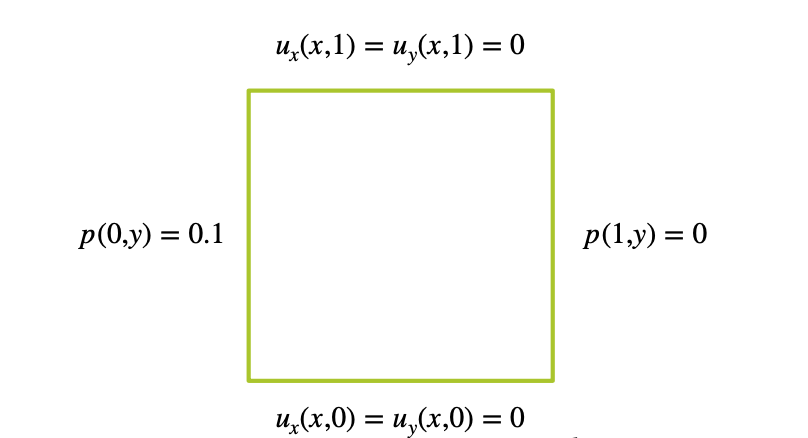
\includegraphics[width=\textwidth]{images/chapter3/stokes_description.png}
	\caption{$\Omega$ and boundary conditions from \eqref{eq:boundary_conditions}}
	\label{fig:stokes_description}\tabularnewline
\end{figure}

In the table \ref{table:stokes_tab} the conditions of the first experiment are described, which includes the use of several simple architectures to approximate the solution. It is important to understand how large a configuration is needed to achieve a certain accuracy. Further, after choosing the architecture, we can talk about using other activation functions to analyze the behavior of the solution.

\begin{table}
	\centering
	\begin{tabular}{| c | c | c |} 
	\hline
		$\vec{n}$ & Parameters number & Accuracy \\ \hline
		$[2, 4, 3]$ & 20 & $0.00489$ \\ \hline
		$[2, 8, 3]$ & 40 & $0.00053$ \\ \hline
		$[2, 16, 3]$ & 70 & $0.00021$ \\ \hline
		$[2, 4, 4, 3]$ & 36 & $0.00195$ \\ \hline
		$[2, 8, 8, 3]$ & 104 & $0.00022$ \\ \hline
		$[2, 16, 16, 3]$ & 334 & $0.00016$ \\ \hline
		$[2, 4, 4, 4, 3]$ & 52 & $0.00076$ \\ \hline
		$[2, 8, 8, 8, 3]$ & 168 & $0.00016$ \\ \hline
		$[2, 16, 16, 16, 3]$ & 592 & $0.00011$ \\ \hline
	\end{tabular}
	\caption{Accuracy of the solution for different number of the parameters [Stokes equation]}
	\label{table:stokes_tab}
\end{table}

From table \ref{table:stokes_tab} it is seen that an increase in the number of parameters in the model leads to an improvement in accuracy almost always, with some caveats: it does not make sense to increase the width of the layers, it makes no sense to increase the number of layers when their width is small.

\begin{figure}
	\centering
	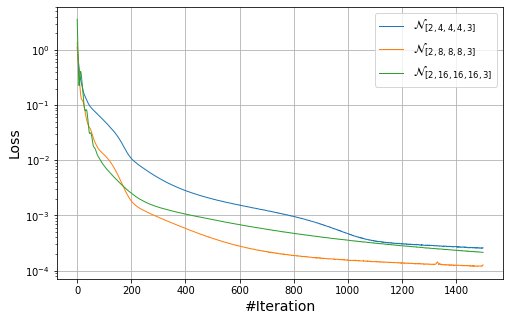
\includegraphics[width=\textwidth]{images/chapter3/stokes_simple_nets_train.png}
	\caption{Training process for ANNs from table \ref{table:stokes_tab}}
	\label{fig:stokes_simple_nets_train}\tabularnewline
\end{figure}

\begin{figure}
	\centering
	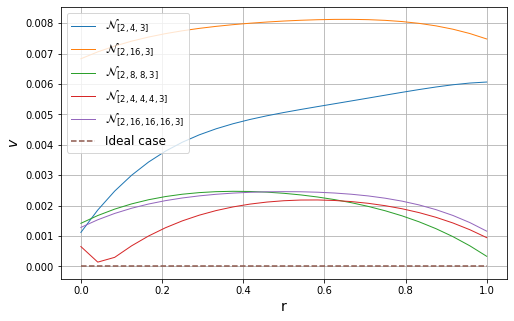
\includegraphics[width=\textwidth]{images/chapter3/stokes_simple_nets_profile.png}
	\caption{Velocity profile for ANNs from table \ref{table:stokes_tab}}
	\label{fig:stokes_simple_nets_profile}\tabularnewline
\end{figure}

\begin{figure}
	\centering
	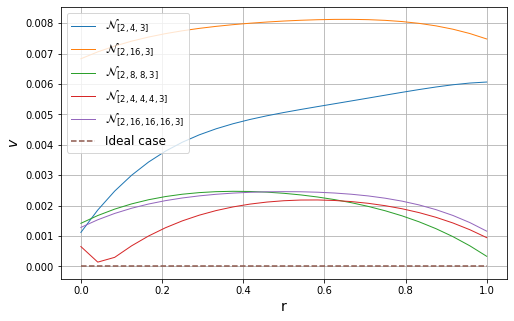
\includegraphics[width=\textwidth]{images/chapter3/stokes_simple_nets_profile_error.png}
	\caption{Velocity profile error for ANNs from table \ref{table:stokes_tab}}
	\label{fig:stokes_simple_nets_profile_error}\tabularnewline
\end{figure}

\begin{figure}
	\centering
	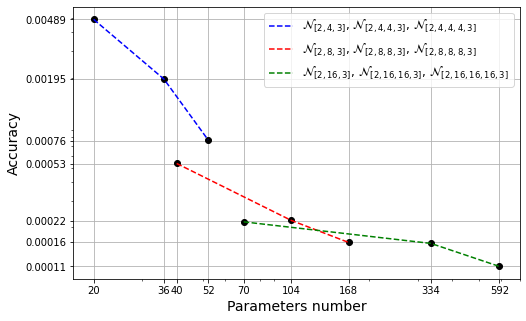
\includegraphics[width=\textwidth]{images/chapter3/stokes_simple_nets_description.png}
	\caption{Parameters number vs Accuracy, description of the table \ref{table:stokes_tab}}
	\label{fig:stokes_simple_nets_description}\tabularnewline
\end{figure}

An important result of table \ref{table:stokes_tab} and figure \ref{fig:stokes_simple_nets_description} is the fact that it is now clear that the optimal architecture for such an equation should not include more than 3 layers of width 8. What does this mean? Answer: the number of parameters greater than 104 with an architecture of $\mathcal{N}_{[2, 8, 8, 3]}$ is optimal. Further, the question will be posed differently: is it possible with an already fixed architecture using activation functions like cosine or Chebyshev polynomials to build an even more accurate solution.

\begin{figure}
	\centering
	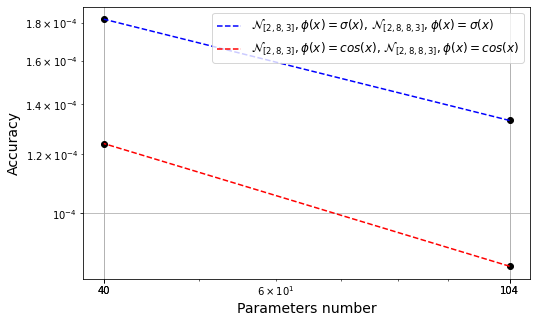
\includegraphics[width=\textwidth]{images/chapter3/stokes_simple_nets_cos.png}
	\caption{Parameters number vs Accuracy, description of the table \ref{table:stokes_tab}}
	\label{fig:stokes_simple_nets_cos}\tabularnewline
\end{figure}

The learning process was depicted for all architectures, as this would lead to a misunderstanding of the drawing due to its overcrowding. Also, an important result is that the architecture using the сosine activation function gave an increase compared to the usual sigmoid function. 

Having chosen about the optimal architecture of the neural network to solve the equation, we can compare whether the improvement of the approximation ability gives the replacement of the activation function within a fixed network configuration. Figure \ref{fig:stokes_simple_nets_cos} shows that there is a change in quality for the better, the calculation was carried out more than 10 times for each model in order to collect statistically significant results. The analytical form of the solution obtained for the figure, respectively:
\begin{equation*}
	\begin{matrix}
		\mathcal{N}_{[2, 8, 3]}^{\sigma} = A^1 \sigma \left [ A^0 x + b^0 \right ] + b^1 \\[10pt]
		\mathcal{N}_{[2, 8, 3]}^{cos} = A^1 cos \left [ A^0 x + b^0 \right ] + b^1
	\end{matrix}
\end{equation*}

It is important to remember that not only the replacement of the activation function was used, but also the criterion \eqref{eq:regularization_criterion_fourier}, \eqref{eq:regularization_criterion_fourier_matrix} corresponding to it, which guaranteed the orthogonality of the functions obtained on the last layer:
\begin{equation*}
	\begin{split}	
		\mathcal{L}_{\text{regularization}} = \left [ \dfrac{sin(W - W^T) + B - B^T}{2 W - 2 W^T} + \dfrac{sin(W + W^T) + B + B^T}{2 W + 2 W^T} - I \right ]_F
	\end{split}
\end{equation*}
